\documentclass[11pt,letterpaper]{article}
\usepackage{fullpage}
\usepackage[pdftex]{graphicx}
\usepackage{amsfonts,eucal,amsbsy,amsopn,amsmath}
\usepackage{url}
\usepackage[sort&compress]{natbib}
\usepackage{natbibspacing}
\usepackage{latexsym}
\usepackage{wasysym} 
\usepackage{rotating}
\usepackage{fancyhdr}
\DeclareMathOperator*{\argmax}{argmax}
\DeclareMathOperator*{\argmin}{argmin}
\usepackage{sectsty}
\usepackage[dvipsnames,usenames]{color}
\usepackage{multicol}
\definecolor{orange}{rgb}{1,0.5,0}
\usepackage{multirow}
\usepackage{sidecap}
\usepackage{caption}
\renewcommand{\captionfont}{\small}
\setlength{\oddsidemargin}{-0.04cm}
\setlength{\textwidth}{16.59cm}
\setlength{\topmargin}{-0.04cm}
\setlength{\headheight}{0in}
\setlength{\headsep}{0in}
\setlength{\textheight}{22.94cm}
\allsectionsfont{\normalsize}
\newcommand{\ignore}[1]{}
\newenvironment{enumeratesquish}{\begin{list}{\addtocounter{enumi}{1}\arabic{enumi}.}{\setlength{\itemsep}{-0.25em}\setlength{\leftmargin}{1em}\addtolength{\leftmargin}{\labelsep}}}{\end{list}}
\newenvironment{itemizesquish}{\begin{list}{\setcounter{enumi}{0}\labelitemi}{\setlength{\itemsep}{-0.25em}\setlength{\labelwidth}{0.5em}\setlength{\leftmargin}{\labelwidth}\addtolength{\leftmargin}{\labelsep}}}{\end{list}}

\bibpunct{(}{)}{;}{a}{,}{,}
\newcommand{\nascomment}[1]{\textcolor{blue}{\textbf{[#1 --NAS]}}}


\pagestyle{fancy}
\lhead{}
\chead{}
\rhead{}
\lfoot{}
\cfoot{\thepage~of \pageref{lastpage}}
\rfoot{}
\renewcommand{\headrulewidth}{0pt}
\renewcommand{\footrulewidth}{0pt}


\title{11-712:  NLP Lab Report}
\author{Bo Lei}
\date{April 26, 2013}

\begin{document}
\maketitle
\begin{abstract}
This paper is the report for CMU 11-712 NLP-lab. Bofinger is a French morphological analyser that is going to be developed in this course.
\end{abstract}


\section{Basic Information about French}

Frech is a Romance language. It is one of the most popular language over the world and is majority spoken by French people. The other areas where French is spoken as a First language are: Belgium, Quebec, Swizerland and Cote d'Ivore etc.\\
\\
There are many types of morphology in French words. For example, the morphology of French verbs can be divided into 3 groups:\\

\indent\indent The first group consists of the verbs that end with "er"\\
\indent\indent The second group consists of the verbs that end with "ir"\\
\indent\indent The third group contains irregular verbs.\\
\\
Each of the verb is subject to change according to the tense (present, past etc).\\
\\
French nouns have gender (masculin ou feminin) and number. This is indicated by the determinant. \\
\\
Adjectives and adverbs also change their number and sex according to the noun that they decorate.
\\
There are rules for each kind of inflection. However exceptions also exist in each case.


\section{Past Work on the Morphology of French}
Many works have been done on French Morphology. For instance, Xerox Morphological Analysis is a commercial NLP tool that supports the analysis of multiple languages including French. It is a mature application and of high accuracy.\\
\\
The Lefff\footnote{http://www.labri.fr/perso/clement/lefff/} is a freely available and large-coverage morphological and syntactic lexicon for French developed by Benoˆıt Sagot. \\
\\
In addition, Morphalou\footnote{http://cnrtl.fr/lexiques/morphalou/} is also a Lexical Markup Framework based model for morphological lexicon, developed by Centre National de Ressources Textuelles et Lexicales. 

\section{Available Resources}

Wikipedia:\\
\indent Wikipedia is a great place for the French language grammar reference. It contains a set of articles describing the complete French word inflection rules\footnote{https://en.wikipedia.org/wiki/French\_verbs} .\\
\\
La Bibliothèque Universelle (ABU)\footnote{http://abu.cnam.fr/}:\\
\indent ABU comprises a great reference for French words morphology and text corpora. It contains the morphology of than 300,000 common used words\footnote{http://abu.cnam.fr/DICO/}. In addition, it also holds 288 texts from 101 authors. To ensure that the corpora are of the same quality (e.g word use, grammar, misspelling) and formalism, I'll choose corpora from Alexandre Dumas's novel Les Trois Mousquetaires (The Three Musketeers). Corpus A will be the first 1000 words, corpus B will be the following 1000 word and Corpus C will be the following 10,000 words.\\
\\
Morphalou:\\
\indent Mentioned above, Morphalou contains a LMF defined lexicon that is almost available for being used as the fundamental of our software.\\

\section{Survey of Phenomena in French}
French verbs:\\
Similar to English, French verbs are conjugated according to the sentence information by adding different suffix after the word stem.\\
\\
Following sentence information may affect how a verb is conjugated:\\
\\
\indent Mood: There are almost seven different moods in French. However some of them are almost not used in contemporary French. For the first round development, I'll focus only on the four most important moods: indicative, subjunctive, conditional and imperative.\\
\\
\indent Tense: Depending on the mood, verbs are conjugated by the tense of the sentence. For indicative, there are eight tenses: present, present perfect, imperfect, pluperfect, simple past, past perfect, simple future and future perfect. For subjunctive, there are four tenses: present, past, imperfect and pluperfect. For imperative, two kinds of tenses exist: present and past. Conditional is special, it has only one type of conjugation regardless the tense.\\
\\
\indent Person: Based on the person, verbs adopts different forms in many cases.\\
\\
French verbs are categorized into three groups. Each group has a different spelling rule. Here lists the spelling rule for each of the group:\\
\\
\indent The first group verbs ends with "er". The spelling rule is defined by replacing "er" with the following letters:\\
\indent past participle: -\'e
\indent present participle: -ant
\indent - indicative\\
\indent\indent present: -e, -es, -e, -ons, -ez, -ent\\
\indent\indent simple past: -ai, -as, -a, -\^ames, -\^ates, -\`erent\\
\indent\indent imperfect: -ais, -ais, -ait, -ions, -iez, -aient\\
\indent\indent simple future: -erai, -eras, -era, -erons, -erez, -eront\\
\\
\indent - subjunctive\\
\indent\indent present: -e, -es, -e, -ions, -iez, -ent\\
\indent\indent imperfect: -asse, -asses, -\^at, -assions, -assiez, -assent\\
\\
\indent - imperative\\
\indent\indent present: N/A, -e, -e, -ons, -ez, -ent\\
\\
\indent - conditional\\
\indent\indent -erais, -erais, -erait, -erions, -eriez, -eraient\\
\\
\indent The second group verbs are those with the ending "ir":\\
\indent past participle: -i
\indent present participle: -ant
\indent - indicative\\
\indent\indent present: -e, -es, -e, -ons, -ez, -ent\\
\indent\indent simple past: -is, -is, -it, -\^imes, -\^ites, -irent
\indent\indent imperfect: -ais, -ais, -ait, -ions, -iez, -aient\\
\indent\indent simple future: -irai, -iras, -ira, -irons, -irez, -iront\\
\\
\indent - subjunctive\\
\indent\indent present: -e, -es, -e, -ions, -iez, -ent\\
\indent\indent imperfect: -isse, -isses, -\^it, -issions, -issiez, -issent\\
\\
\indent - imperative\\
\indent\indent present: N/A, -is, -isse, -issons, -issez, -issent\\
\\
\indent - conditional\\
\indent\indent -irais, -irais, -irait, -irions, -iriez, -iraient\\
\\
\indent The theird group verbs are special cases which do not have a common spelling rule. Fortunately there are not many verbs falling into this group. We can treat them case by case.\\
\\
French nouns:\\
Each french noun has a gender (masculine or feminine). Most of the time, different genders of a same word are of different spelling. Most of the feminine forms of a nouns adds a "e" at the end of its masculine form. Like English, some French nouns are countable and some are uncountable. Generally, the plural form of a countable noun adds a "s" at the end. But sometimes "x", "eux" may be added. There are also irregular plural forms such as "yeux" as the plural form of "\oe il" (the word "eye" in English).\\
\\
French adjectives:\\
Adjectives in French also need to conform the gender of the sentence.\\
\\
French articles and determiners:\\
\indent definite article:\\
\indent\indent Singular: le (masculine), la (feminine)\\
\indent\indent plural: les\\
\indent indefinite article:\\
\indent\indent Singular: un (masculine), une (feminine)\\
\indent\indent plural: des\\
\indent partitive article:\\
\indent\indent Singular: du (masculin), de la (feminine)\\
\indent\indent plural: des\\
\\
There are also types of words in French such as Pronoun, adverbs, Prepositions, Negation words which do not have complex spelling rules. Our program will treat them in a lower priority.

\section{Initial Design}
\subsection*{System architecture}
Following is a big picture of the system.\\
\centerline{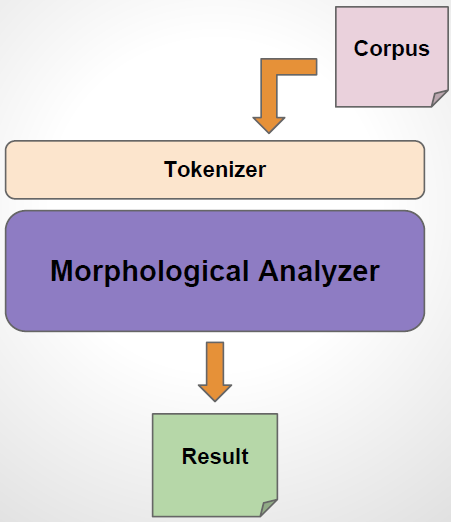
\includegraphics[width=60mm]{img/overview.png}}\\
The raw corpus is first tokenized by a tokenizer, then the analyser will do the morphological analysis on the tokenized corpus.\\


The analyser can be divided by word types:\\
\indent Lexicon: This will be the module that defines all the original form of the French words and third regular inflection. It includes\\
\begin{itemize}
\item Nouns
\item Verbs
\item Adjectives \& Adverbs
\item Articles
\item Determiners
\item Conjunctions
\item Negations
\item Prepositions
\item Pronouns
\end{itemize}
The list of words come from Wikitionary\footnote{https://en.wiktionary.org/wiki/Index:French}.

\indent Irregular forms: All the exceptions of the regular conjugations are handled in this module.\\

The structure of analyser can be illustrated by the following figure.\\
\centerline{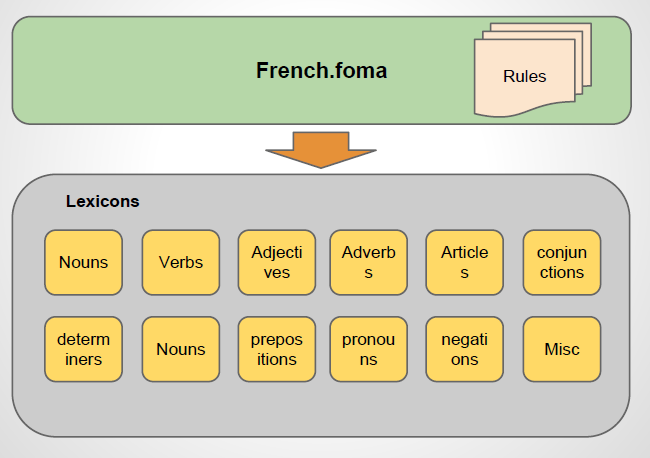
\includegraphics[width=100mm]{img/analyser.png}}\\

\section{System Analysis on Corpus A}
At this point, I have implemented a part of word categories in French. They are:\\
\begin{itemize}
\item Nouns
\item Verbs
\item Adjectives \&  Adverbs
\item Articles
\item Determiners

\end{itemize}
Except for 3rd group verbs, Only regular inflections were implemented.\\
\\
This is a pilot version and its purpose is only to check if the system is able to analyse something. As a result, the main evaluation criterion is its recognition rate, namely the percentage of the words that it is able to recognize and give some parse.\\
\\
So the program is run on Corpus A, the first 1000 words from Les Trois Mousquetaires. Then a python script is used to do the evaluation on the result.
\\
\begin{verbatim}
word type count:
497
word type recognition rate:
0.64185110664
============
word token count:
1224
word token recognition rate:
0.646241830065
\end{verbatim}

\section{Lessons Learned and Revised Design}
In this round of development, the most important thing I learned is how to use Foma to implement a FST based morphological analyser. \\
\\
At the beginning I didn't know how to separate different kinds of words so I put everything into one big file. As I get more familiar with Foma, I was able to divide the lexicons according to their category. The separation does not only makes sense in terms of system architecture, but also makes it easier to debug because each module can become a standalone FST.\\
\\
Some tricks are used. For example, French regular verbs (1st and 2nd groups) end with a certain suffix. So it is easier for the lexicon file to keep track of the stem and the suffix separately.\\
\\
In the next step, I plan to finish adding all kinds of French vocabularies:\\
\\
\begin{verbatim}
Prepositions
Pronouns
Negation
\end{verbatim}
Also, the system should be case insensitive.\\
\section{System Analysis on Corpus B}
In the second round of development, Prepositions, Pronouns and Negation are added into the analyser. By far, almost all french word types has been covered. Again, the recognition rate is calculated.\\

\begin{verbatim}
word type count:
471
word type recognition rate:
0.717622080679
============
word token count:
1163
word token recognition rate:
0.798796216681
\end{verbatim} 
After examining the unrecognised words, There are two major reasons that the analyser doesn't recognize words:\\
\begin{itemize}
\item Many common words such as pr\`es, et, o\`u etc. are not recognized. This is because obviously some important words are either not included in the lexicon or wrongly spelled.
\item Tokens that contain capitalized alphabets are not recognized. This is because so far the analyser is case sensitive. It would be good to make it case insensitive. Because the analyser is supposed to treat tokens in the same way regardless its case.
\end{itemize}
\section{Final Revisions}
Further improvement has been made in this round of development.
\begin{itemize}
\item Case insensitive
The corpus always contains words with capitalized alphabets. For example all leading word of a sentence starts with a capitalized letter. Obviously they should be considered correct and the analyser is supposed to give a parse.
\item Ignoring accents\\
In human text, people tent to miss use accents.For example, \`a Paris (in Paris) is always written as a Paris. Even without typo, both \`a and a will become A when appear at the beginning of a sentence. Thus, it is decided that the analyser will ignore accents.
\item improved the lexicon
\end{itemize}
Corpus C is contains chapter 11 to 13 in Les Trois Mousquetaires.\\
\begin{verbatim}
word type count:
2639
word type recognition rate:
0.857521788556
============
word token count:
15668
word token recognition rate:
0.938026550932
\end{verbatim} 
\section{Future Work}
Up to now, most of the basic French inflections are implemented. However there are much more things left to be done.
\begin{itemize}
\item Fixing bugs and Improving the lexicon
It is inevitable that the program has bugs. Some inflection rules may not be correctly defined. Also in reviewing the unrecognised words, I found that there are common used words not included in the lexicon.
\item Handling more irregular inflections\\
Most of the effort has been made in dealing with 3rd group verbs. There are other irregular inflections left unimplemented.
\item Better evaluation mechanism\\
So far the evaluation script only calculates the recognition rate on the analysis result. It is desired to evaluate the precision and recall of the analyser.
\end{itemize}
\section{Appendix}
\subsection*{List of tags}
\begin{table}
    \begin{tabular}{ll}
		+Adj & Adjective \\
		+Adv & Adverb \\
		+Con & Conditional \\
		+Conjun & Conjunction \\
		+DefArt & Definite article \\
		+DemDet & Demonstrative determiners \\
		+Demo & Demonstrative pronouns \\
		+Det & determiners \\
		+DirObj & Direct Object Pronouns \\
		+Disj & Disjunctive Pronouns \\
		+Fem & feminine \\
		+Fut & Simple future \\
		+Impr & Imperative \\
		+Ind & Indicative \\
		+IndefArt & Indefinite article \\
		+IndirObj & Indirect-object pronouns \\
		+Inf & infinitive \\
		+Intero & Interrogative pronouns \\
		+InterrDet & Interrogative determiners \\
		+Mas & masculine \\
		+Neg & negations \\
		+Nom & nouns \\
		+Num & numbers \\
		+PartArt & partitive article \\
		+Person & Personal Pronouns \\
		+Pl & plural \\
		+Poss & Possessive pronouns \\
		+PossDet & Possessive determiners \\
		+PP1P & First person plural \\
		+PP1S & First person singular \\
		+PP2P & Second person plural \\
		+PP2S & Second person singular \\
		+PP3P & Third person plural \\
		+PP3S & Third person singular \\
		+PPas & Past Partical \\
		+PPre & Present Partical \\
		+Pre & present \\
		+Prep & prepositions \\
		+Pron & pronouns \\
		+PSim & Simple past \\
		+Refl & Reflexive pronouns \\
		+Sg & singular \\
		+Sub & subjunctive \\
		+Subj & Subject pronouns \\
		+Ver & Verb \\
    \end{tabular}
\end{table}
\bibliographystyle{plainnat}
\bibliography{refs}
\label{lastpage}
\end{document}
